\subsection{Deducción y descripción del método}
\subsubsection{Deducción}
En el método de Newton Raphson, se necesita saber la derivada de la función en cada aproximación. La fórmula para hallar el siguiente punto en dicho método es la siguiente:

\begin{equation}
\label{secant_eq1}
p_n = p_{n-1} - \frac{f(p_{n-1})}{f'(p_{n-1})}
\end{equation} 

Conocer la derivada de la función puede resultar más complejo, por lo que, en lugar de la derivada, se puede utilizar la siguiente aproximación:

\begin{gather*}
f'(p_{n-1}) = \lim_{x\to p_{n-1}} \frac{f(x) - f(p_{n-1})}{x-p_{n-1}} 
\end{gather*}

Si $P_{n-2}$ está cerca de $P_{n-1}$, entonces tenemos lo siguiente:

\begin{gather*}
f'(p_{n-1}) \approx \frac{f(p_{n-2})-f(p_{n-1})}{p_{n-2}-p_{n-1}} = \frac{f(p_{n-1})-f(p_{n-2})}{p_{n-1}-p_{n-2}}
\end{gather*}

Al sustituir la aproximación de $f'(P_{n-1})$ en la fórmula \refeq{secant_eq1}, tenemos la fórmula del método de la secante \cite{Burden_English}:

\begin{gather*}
p_n = p_{n-1} - \frac{f(p_{n-1})}{\frac{f(p_{n-1})-f(p_{n-2})}{p_{n-1}-p_{n-2}}}
\end{gather*}

\begin{equation}
    \label{secant_eq2}
p_n = p_{n-1} - \frac{f(p_{n-1})(p_{n-1}-p_{n-2})}{f(p_{n-1})-f(p_{n-2})} 
\end{equation}


A diferencia de Newton, en el método de la secante se necesitan dos puntos iniciales $P_{n-2}$ y $P_{n-1}$. Al utilizar la fórmula de la secante, se encuentra el siguiente punto Pn. 

Después se modifica la notación para encontrar $P_{n+1}$ utilizando los dos puntos anteriores $P_{n-1}$ y $P_n$, y así sucesivamente hasta encontrar la raíz.

\subsubsection{Descripción}
El método de la secante sirve para encontrar raíces de ecuaciones sin saber la derivada de la función (a diferencia del método de Newton en dónde sí es necesario conocer la derivada). La raíz de una ecuación no es otra cosa más que el valor de la $X$ cuando $f(x)$ vale cero. Es decir que este método es una modificación del método de Newton.

¿Cómo funciona?

El método de la secante requiere dos puntos iniciales $P_{n-2}$ (valor más pequeño) y $P_{n-1}$ (valor más grande). Esos dos valores sirven para generar una línea recta que va a cruzar con el eje de las $X$ y justamente ese punto se va a conocer como $P_n$ o la aproximación a la raíz.

Después de utilizar la fórmula para encontrar $P_n$, se modifica la notación para encontrar $P_{n+1}$ utilizando los dos puntos anteriores $P_{n-1}$ y $P_n$, y así sucesivamente hasta encontrar la raíz o al menos hasta que el error sea menor o igual a la tolerancia. 

No se necesita otra cosa más que la función y proponer los dos valores de inicio para tener la aproximación. A diferencia del método de newton, no se ocupa la derivada.


\subsection{Análisis del error y demostración de convergencia}

Se asume que $r$ es una raíz para $f(x)=0$. La secuencia ${x_n}$ del método de la secante está dada por: 

\begin{gather*}
x_{n+1 }= x_{n} - \frac{f(x_{n})(x_{n}-x_{n-1})}{f(x_{n})-f(x_{n-1})} 
\end{gather*}

Se quiere encontrar el exponente $p$ de tal manera que:

\begin{gather*}
\lim_{n\to \infty} \frac{|x_{n+1}-r|}{|x_n - r|^{p}} = \lim_{n\to \infty} \frac{|e_{n+1}|}{|e_n|^{p}} = \lambda
\end{gather*}

En donde $e_n = x_n - r$. Por el teorema de Taylor,

\begin{gather*}
f(x_{n-1})= f(e_{n-1}+r) = f(r)+e_{n-1}f'(r) \\
+\frac{e^{2}_{n-1}}{2}f''(r)+O(e^{3}_{n-1})
\end{gather*}

\begin{gather*}
f(x_{n})= f(e_n+r) = f(r)+e_{n}f'(r)+\frac{e^{2}_n}{2}f''(r)+O(e^{3}_n)
\end{gather*}

Ya que $f(r)=0$, se tiene para $e=e_n$ o $e=e_{n-1}$

\begin{gather*}
f(e+r)= e f'(r)+\frac{e^{2}}{2}f''(r)+O(e^{3})
\end{gather*}

\begin{gather*}
f(e+r) \approx e f'(r)+\frac{e^{2}}{2}f''(r)
\end{gather*}

El método de la secante da:

\begin{gather*}
x_{n+1 }= x_{n} - \frac{f(x_{n})(x_{n}-x_{n-1})}{f(x_{n})-f(x_{n-1})} 
\end{gather*}

\begin{gather*}
\Rightarrow e_{n+1}+r= e_{n} + r - f(e_n + r) \frac{(e_n +r) -(e_{n-1}+r)}{f(e_n + r)-f(e_{n-1} + r)} 
\end{gather*}

\begin{equation}
    \label{secant_eq3}
\Rightarrow e_{n+1}= e_{n} - \frac{f(e_n + r)(e_n - e_{n-1})}{f(e_n + r)-f(e_{n-1} + r)} 
\end{equation}\\

Dejando:\\

\begin{gather*}
M= \frac{f''(r)}{2f'(r)} \Leftrightarrow \frac{f''(r)}{2} = Mf'(r)
\end{gather*}\\\\

Ignorando los términos de orden superior, el numerador de la ecuación \refeq{secant_eq3} se convierte en lo siguiente:

\begin{gather*}
    f(e_n +r)(e_n - e_{n-1})= (e_nf'(r)+\frac{e^{2}_n}{2}f''(r))(e_n -e_{n-1}) \\
    = (e_nf'(r)+Me^{2}_nf'(r))(e_n -e_{n-1}) \\
    = e_nf'(r)(1+Me_n)(e_n -e_{n-1})
\end{gather*} 

El denominador de la ecuación \refeq{secant_eq3} se convierte en:


\begin{gather*}
    f(e_n +r)-f(e_{n-} +r)= [e_nf'(r)+\frac{1}{2}f''(r)e^{2}_n][e_{n-1}f'(r) \\
    +\frac{1}{2}f''(r)e^{2}_{n-1}] \\
    = f'(r)(e_n-e_{n-1})+\frac{1}{2}f''(r)(e^{2}_n -e^{2}_{n-1}) \\
    = f'(r)(e_n-e_{n-1})+Mf'(r)(e^{2}_n -e^{2}_{n-1}) \\
    = f'(r)(e_n-e_{n-1})(1+M(e_n +e_{n-1})) \\
\end{gather*}


Por lo tanto, la ecuación \refeq{secant_eq3} ahora es:


\begin{gather*}
    e_{n+1}= e_{n} - \frac{e_nf'(r)(1+Me_n)(e_n -e_{n-1})}{f'(r)(e_n-e_{n-1})(1+M(e_n +e_{n-1}))} \\
    = e_{n} - \frac{e_n(1+Me_n)}{1+M(e_n+e_{n-1})} \\
    = \frac{e_n+e_n M(e_n+e_{n-1})-e_n(1+Me_n)}{1+M(e_n+e_{n-1})} \\
    = \frac{M e_n e_{n-1}}{1+M(e_n+e_{n-1})} \\
\end{gather*}


Lo cual implica que:

\begin{gather*}
    e_{n+1} \approx M e_n e_{n-1} \approx \frac{f''(r)}{2f'(r)} e_n e_{n-1}
\end{gather*}

Ahora se calcula el exponente $p$. Se tiene $|e_{n+1}= \lambda|e_n|^{p}$ y $|e_{n+1} \approx |M||e_n||e_{n-1}|$, entonces:

\begin{gather*}
    \lambda|e_n|^{p}=|M||e_n||e_{n-1}| \\
    \Rightarrow |e_n|^{p-1}=|M/\lambda||e_{n-1}| \\
    \Rightarrow |e_n|=|M/\lambda|^{1/{p-1}}|e_{n-1}|^{1/{p-1}}= \lambda|e_{n-1}|^{p} \\
\end{gather*} 

Por lo que se obtiene \cite{edwards}:

\begin{gather*}
    p=\frac{1}{p-1} \Rightarrow p^{2}-p-1=0 \Rightarrow p = \frac{1+ \sqrt{5}}{2}
\end{gather*} 

La convergencia de este método es superlineal, lo que significa que es mayor que los de convergencia linear pero menor que los de convergencia cuadrática como el método de Newton.

En este caso, $p$ es el número de oro, aproximadamente $1.618$, lo que significa que el método de la secante es casi tan rápido como Newton-Raphson pero un poco más lento y que es más rápido que los de convergencia lineal.

\subsection{Análisis sobre la eficiencia del método}

El método de la secante es iterativo, requiere la función y los dos puntos anteriores para encontrar $Pn$ o la raíz, utiliza la recta secante que pasa por los puntos que le corresponden a las aproximaciones anteriores y puede resultar más fácil de utilizar a comparación del método de Newton, sin embargo el método de la secante no siempre converge, es decir que no necesariamente se encontrará una aproximación de la solución que se está buscando.  Además, no necesariamente se tiene una referencia al elegir los dos puntos iniciales y si estos no son ideales, el método no resultará muy eficiente. 

Como se mencionó anteriormente, el método puede diverger como por ejemplo, si se tienen dos puntos iniciales ($X_0$ y $X_1$), se calculan sus imágenes y la recta que los contiene, y como resultado se obtiene una recta paralela al eje $x$, es decir, una recta que nunca va a interceptar al eje $x$, en este caso el método diverge. Algebraicamente, se estaría obteniendo una división entre cero. También se pueden tener variaciones de eso, no obteniendo una recta paralela exactamente al eje $x$, pero que se va a interceptar en el infinito, en un número muy grande o muy pequeño.


Otro caso de divergencia es cuando en lugar de irse acercando a la solución que se busca, más bien se está alejando. Gráficamente es muy sencillo ver cuándo el método va a diverger, porque no nos estamos acercando al cero, es decir, a la intercepción de la función con el eje $x$. Algebraicamente, se debe ver si el error está aumentando o disminuyendo. Si el error disminuye, el método está convergiendo y si está aumentando entonces el método probablemente esté divergiendo. 


\subsection{Ventajas y desventajas}

\subsubsection{Ventajas}

\begin{itemize}
  \item En el método de Newton, se ocupa la derivada de la función lo cual resulta en más operaciones aritméticas y se vuelve más complejo. A diferencia del método de Newton, en el método de la secante no se ocupa la derivada de la función.
  \item Solo se necesita conocer la función y proponer dos puntos iniciales, se sustituyen en la función y lo mismo se repite hasta encontrar la raíz.
  \item Es menos complejo que otros métodos que requieren más pasos y operaciones para obtener resultados.
\end{itemize}

\subsubsection{Desventajas}

\begin{itemize}
  \item La convergencia del método de la secante es ligeramente más lenta que la del método de Newton. 
  \item Un problema que se tiene con la aplicación del método de la secante es la posibilidad de que el polinomio tenga raíces complejas incluso cuando todos los coeficientes son números reales. 
  \item La agrupación de raíces no está garantizada para el método de la secante.
  \item Se necesitan dos valores iniciales, entonces tenemos más probabilidad de que este método numérico no sea convergente. Al contrario, Newton al solo tener un valor inicial Xo tiene más probabilidad de converger.
  \item No siempre converge, es decir que no necesariamente se va a encontrar una aproximación de la solución que estamos buscando.
  \item El método depende mucho de las condiciones iniciales que se escojan.
\end{itemize}

\subsection{Pseudocódigo}

\begin{algorithm}
    \SetKwComment{Comment}{/}{/}
    
    \caption{Método de la secante} 
    \KwIn{Aproximaciones iniciales $p_0$, $p_1$ tolerancia TOL; número máximo de iteraciones $N_0$.}\
    \KwOut{Solución aproximada \textit{p} o mensaje de error.}
    $i = 2$; 
    \BlankLine
    $q_0 = f(p_0)$; 
    \BlankLine
    $q_1 = f(p_1)$.
    \BlankLine
    \While{$i \le n_0 $}{
        $p = p_1 - q_1(p_1 - p_0)/(q_1-q_0)$
        \If{$|p-p_1| < TOL$}{\tcp{El procedimiento fue exitoso} \Return{p}}
        $i = i + 1$.
        $p_0=p_1$; 
        $q_0=q_1$;
        $p_1=p$;
        $q_1=f(p)$
    }
    \Return \KwOut{"El metodo fallo luego de N iteraciones, N="$N_0$}
    \end{algorithm}

\subsection{Elementos ilustrativos}

Ejemplo gráfico del método de la secante con la función $f(x)=x^2-1$:\\

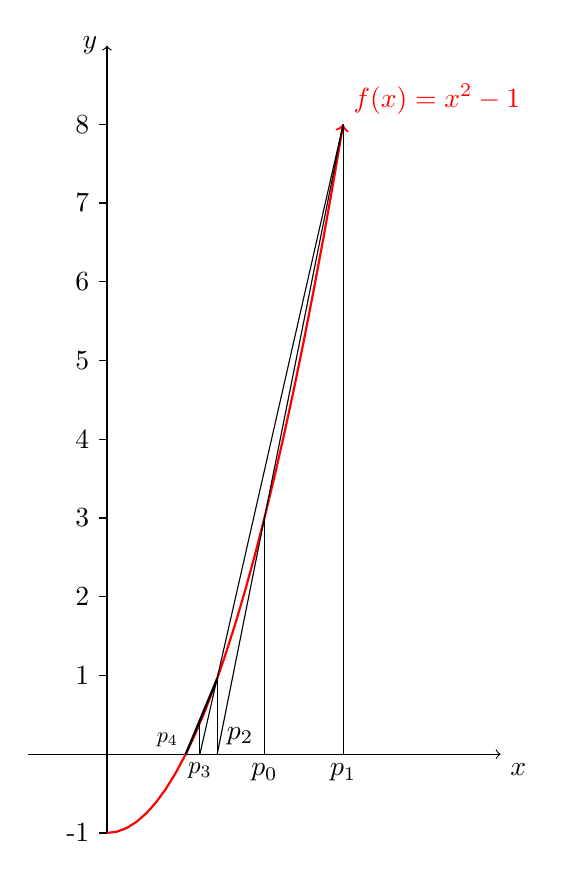
\begin{tikzpicture}[domain=0:2]
    \draw[->] (-1,0) -- (5,0)
    node[below right] {$x$};
    \draw[->] (0,-1) -- (0,9)
    node[left] {$y$};
    \foreach \y in {-1,1,2,3,4,5,6,7,8}
    \draw (0,\y) -- (-0.1,\y) node[left] {\y};
    
    \draw[red,thick,->] plot[domain=0:3] (\x,\x^2-1) 
    node[above right] {$f(x) = x^2-1$};
    
     \coordinate (A) at (2,0);
     \node[below] at (2,0) {$p_0$};
     \coordinate (B) at (3,0);
     \node[below] at (3,0) {$p_1$};
     \coordinate (C) at (1.4,0);
     \node[above right] at (1.4,0) {$p_2$};
     \coordinate (D) at (1.18,0);
     \node[below, scale=0.9] at (1.18,0) {$p_3$};
     \coordinate (E) at (1.00,0);
     \node[above left, scale=0.8] at (1.00,0) {$p_4$};
     \coordinate (F) at (2,3);
     \coordinate (G) at (3,8);
     \coordinate (H) at (1.4,0.96);
     \coordinate (I) at (1.18,0.3924);
     
    \draw (A) -- (F);
    \draw (B) -- (G);
    \draw (G) -- (C);
    \draw (C) -- (H);
    \draw (G) -- (D);
    \draw (D) -- (I);
    \draw[thick] (H) -- (E);
    
\end{tikzpicture}


\subsection{Ejemplos}

\subsubsection{Ejemplo 1}

Utilice el método de la secante para encontrar una solución para $f(x) = e^{-x} - x$, utilizando como puntos iniciales $p_{n-2} = 2$ y $p_{n-1} = 5$. \\
\\\\
\begin{tabularx}{0.4\textwidth} { 
  | >{\arraybackslash}X 
  | >{\arraybackslash}X
  | >{\arraybackslash}X
  | >{\arraybackslash}X
  | >{\arraybackslash}X | }
 \hline
 i & $p_{n-1}$ & $p_{n-2}$ & $f(p_{n-1})$ & $f(p_{n-2})$ \\
 \hline
 1 & 5 & 2 & -4.99 & -1.86 \\
 \hline
 2 & 0.21 & 5 & 0.60 & -4.99 \\
 \hline
 3 & 0.72 & 0.21 & -0.24 & 0.60 \\
 \hline
 4 & 0.58 & 0.72 & -0.02 & -0.24 \\
 \hline
 5 & 0.57 & 0.58 & 0.00 & -0.02 \\
 \hline
\end{tabularx} \\\\

\begin{tabularx}{0.3\textwidth}{ 
  | >{\arraybackslash}X 
  | >{\arraybackslash}X
  | >{\arraybackslash}X | }
 \hline
 i & $p_{n}$ & ErAbs \% \\
 \hline
 1 & 0.21 & 2258.71  \\
 \hline
 2 & 0.72 & 70.69  \\
 \hline
 3 & 0.58 & 25.25  \\
 \hline
 4 & 0.57 & 1.88  \\
 \hline
 5 & 0.57 & 0.00  \\
 \hline
\end{tabularx} \\\\

Fórmula del método de la secante:

\begin{gather*}
p_n = p_{n-1} - \frac{f(p_{n-1})(p_{n-1}-p_{n-2})}{f(p_{n-1})-f(p_{n-2})} 
\end{gather*} \\

En el caso del error, se puede calcular el error absoluto con la siguiente fórmula:

\begin{gather*}
    EA = |\frac{p_n - p_{n-1}}{p_n}|*100
\end{gather*} \\

\paragraph{Iteración 1}
\begin{gather*}
    f(x) = e^{-x} - x \\
    f(p_{n-1}) = e^{-5} - 5 = -4.99 \\
    f(p_{n-2}) = e^{-2} - 2 = -1.86 \\
    p_n = (5)- \frac{(-4.99*(5-2))}{(-4.99-(-1.86))} = 0.21 \\
    Error absoluto = \frac{0.21-5}{0.21}100 = 2258.71
\end{gather*} \\

\paragraph{Iteración 2}
\begin{gather*}
    f(p_{n-1}) = e^{-0.21} - 0.21 = 0.60 \\
    f(p_{n-2}) = e^{-5} - 5 = -4.99 \\
    p_n = (0.21)- \frac{(0.60*(0.21-5))}{(0.60-(-4.99))} = 0.72 \\
    Error absoluto = \frac{0.72-0.21}{0.72}100 = 70.69
\end{gather*} \\

\paragraph{Iteración 3}
\begin{gather*}
    f(p_{n-1}) = e^{-0.72} - 0.72 = -0.24 \\
    f(p_{n-2}) = e^{-0.21} - 0.21 = 0.60 \\
    p_n = (0.72)- \frac{(-0.24*(0.72-0.21))}{(-0.24-(0.60))} = 0.58 \\
    Error absoluto = \frac{0.58-0.72}{0.58}100 = 25.25
\end{gather*} \\

\paragraph{Iteración 4}
\begin{gather*}
    f(p_{n-1}) = e^{-0.58} - 0.58 = -0.02 \\
    f(p_{n-2}) = e^{-0.72} - 0.72 = -0.24 \\
    p_n = (0.58)- \frac{(-0.02*(0.58-0.72))}{(-0.02-(-0.24))} = 0.57 \\
    Error absoluto = \frac{0.57-0.58}{0.57}100 = 1.88
\end{gather*} \\

\paragraph{Iteración 5}
\begin{gather*}
    f(p_{n-1}) = e^{-0.57} - 0.57 = 0.00 \\
    f(p_{n-2}) = e^{-0.58} - 0.58 = -0.02 \\
    p_n = (0.57)- \frac{(0.00*(0.57-0.58))}{(0.00-(-0.02))} = 0.57 \\
    Error absoluto = \frac{0.57-0.57}{0.57}100 = 0.00
\end{gather*} \\

En este ejemplo se puede observar que al utilizar el último $p_n = 0.57$ en la función original, se obtiene $0$, por lo que ya se ha encontrado la raíz. Cabe mencionar que los resultados se han redondeado a dos decimales.


\subsubsection{Ejemplo 2} 
Utilice el método de la secante para encontrar una solución para $f(x) = x^{2} - 3x - 4$, utilizando como puntos iniciales $p_{n-2} = 5$ y $p_{n-1} = 7$. \\\\

\begin{tabularx}{0.4\textwidth} { 
  | >{\arraybackslash}X 
  | >{\arraybackslash}X
  | >{\arraybackslash}X
  | >{\arraybackslash}X
  | >{\arraybackslash}X | }
 \hline
 i & $p_{n-1}$ & $p_{n-2}$ & $f(p_{n-1})$ & $f(p_{n-2})$ \\
 \hline
 1 & 7 & 5 & 24.00 & 6.00 \\
 \hline
 2 & 4.33 & 7 & 1.78 & 24.00 \\
 \hline
 3 & 4.12 & 4.33 & 0.61 & 1.78 \\
 \hline
 4 & 4.01 & 4.12 & 0.04 & 0.61 \\
 \hline
 5 & 4.00 & 4.01 & 0.00 & 0.04 \\
 \hline
\end{tabularx} \\\\

\begin{tabularx}{0.3\textwidth} { 
  | >{\arraybackslash}X 
  | >{\arraybackslash}X
  | >{\arraybackslash}X | }
 \hline
 i & $p_{n}$ & ErAbs \% \\
 \hline
 1 & 4.33 & 61.54  \\
 \hline
 2 & 4.12 & 5.18  \\
 \hline
 3 & 4.01 & 2.81  \\
 \hline
 4 & 4.00 & 0.18  \\
 \hline
 5 & 4.00 & 0.00  \\
 \hline
\end{tabularx} \\\\


\paragraph{Iteración 1}
\begin{gather*}
    f(x) =x^{2}-3x-4 \\
    f(p_{n-1}) =(7)^{2}-3(7)-4 = 24 \\
    f(p_{n-2}) =(5)^{2}-3(5)-4 = 6 \\
    p_n = (7)- \frac{(24*(7-5))}{(24-6)} = 4.33 \\
    Error absoluto = \frac{4.33-7}{4.33}100 = 61.54 
\end{gather*} \\

\paragraph{Iteración 2}
\begin{gather*}
    f(p_{n-1}) =(4.33)^{2}-3(4.33)-4 = 1.78 \\
    f(p_{n-2}) =(7)^{2}-3(7)-4 = 24 \\
    p_n = (4.33)- \frac{(1.78*(4.33-7))}{(1.78-24)} = 4.12 \\
    Error absoluto = \frac{4.12-4.33}{4.12}100 = 5.18
\end{gather*} \\

\paragraph{Iteración 3}
\begin{gather*}
    f(p_{n-1}) =(4.12)^{2}-3(4.12)-4 = 0.61 \\
    f(p_{n-2}) =(4.33)^{2}-3(4.33)-4 = 1.78 \\
    p_n = (4.12)- \frac{(0.61*(4.12-4.33))}{(0.61-1.78)} = 4.01 \\
    Error absoluto = \frac{4.01-4.12}{4.01}100 = 2.81
\end{gather*} \\

\paragraph{Iteración 4}
\begin{gather*}
    f(p_{n-1}) =(4.01)^{2}-3(4.01)-4 = 0.04 \\
    f(p_{n-2}) =(4.12)^{2}-3(4.12)-4 = 0.61 \\
    p_n = (4.01)- \frac{(0.04*(4.01-4.12))}{(0.04-0.61)} = 4.00 \\
    Error absoluto = \frac{4.00-4.01}{4.00}100 = 0.18
\end{gather*} \\

\paragraph{Iteración 5}
\begin{gather*}
    f(p_{n-1}) =(4.00)^{2}-3(4.00)-4 = 0.00 \\
    f(p_{n-2}) =(4.01)^{2}-3(4.01)-4 = 0.04 \\
    p_n = (4.00)- \frac{(0.00*(4.00-4.01))}{(0.00-0.04)} = 4.00 \\
    Error absoluto = \frac{4.00-4.00}{4.00}100 = 0.00
\end{gather*} \\

En este ejemplo se puede observar que al utilizar el último $p_n = 4.00$ en la función original, se obtiene $0$, por lo que ya se ha encontrado la raíz.
